\clearpage

\section{Задача 6: Нелінійні регресії в Python}

\markboth{Задача 6}{}

За умовою використовуємо лише перші 500 продажів та пояснюємо SalePrice
через YearBuilt. У цих двох колонках немає пропусків. Файл упорядкований
за роком продажу, тому ця підвибірка містить лише продажі 2009--2010
років і не є випадковою.


\Needspace{186.0pt}

\subsection{(а) Лінійна модель}

\begin{taskstatement}
Побудуйте двовимірну діаграму розсіювання (bivariate scatter plot) та
оцініть відповідну лінійну (!) модель через statsmodels або
LinearRegression з sklearn. Додайте лінію регресії на графік.
\end{taskstatement}


\pythoncode{p6-c6}

\Needspace{65.19999999999999pt}

\resulttext{p6-c6-out0.txt}

\begingroup\fontsize{7.5}{9.5}\selectfont\setlength{\tabcolsep}{2.5mm}\renewcommand{\arraystretch}{1.15}
\par\vspace{2pt}\noindent\begin{tabular}{|ll|}
\hline
 & Лінійна модель \\
\hline
beta\_0 & -3.45966e+06 \\
beta\_1 (YearBuilt) & 1846.65 \\
SE(beta\_1) & 115.494 \\
t & 15.9893 \\
p & 9.55339e-47 \\
R² & 0.339221 \\
Найстаріший рік & 1875 \\
Його фактична ціна & 94000 \\
Його прогноз & 2818.23 \\
\hline
\end{tabular}\par\vspace{2pt}
\endgroup


\begingroup\fontsize{7.5}{9.5}\selectfont\setlength{\tabcolsep}{2.5mm}\renewcommand{\arraystretch}{1.15}
\par\vspace{2pt}\noindent\begin{tabular}{|llll|}
\hline
Year\allowbreak{}Built & Продажів & Середній залишок, дол. & Частка точок під прямою \\
\hline
(1870, 1950] & 79 & 22519.3 & 0.329114 \\
(1950, 1980] & 185 & -25041.8 & 0.8 \\
(1980, 2000] & 93 & -4279.42 & 0.645161 \\
(2000, 2010] & 143 & 22739.1 & 0.524476 \\
\hline
\end{tabular}\par\vspace{2pt}
\endgroup


\begin{figure}[H]
\centering
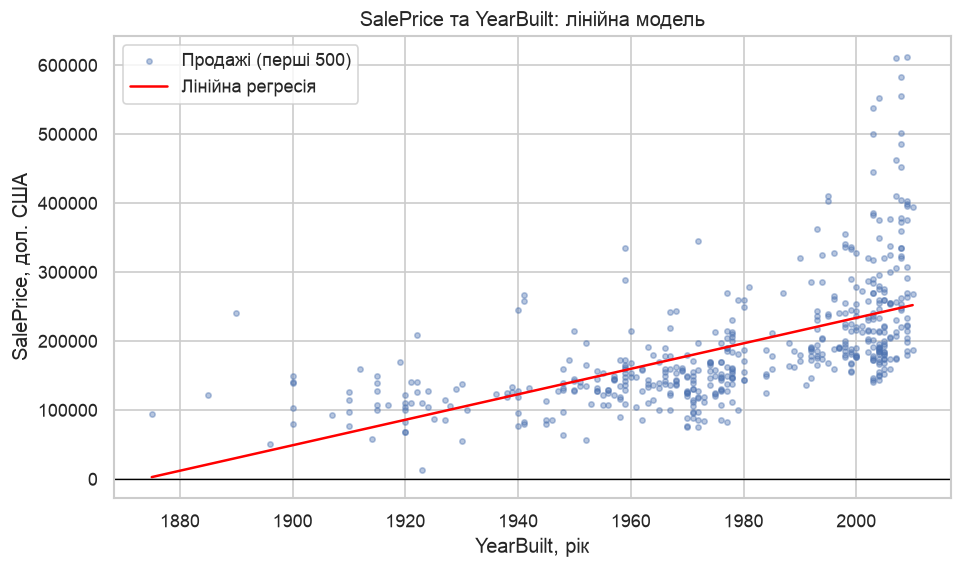
\includegraphics[width=\linewidth,height=0.82\textheight,keepaspectratio]{../../figures/problem6_linear.png}
\caption{Лінійна модель для перших 500 продажів.}
\end{figure}


\answerheading
Модель: \(SalePrice_i=\beta_0+\beta_1 YearBuilt_i+\varepsilon_i\), де
\(\beta_0\) позначає вільний член, \(\beta_1\) нахил, \(\varepsilon_i\)
похибку продажу \(i\); оцінена МНК через \texttt{statsmodels}.

\begin{itemize}
\item
  \(\widehat\beta_1=1846.65\) (\(SE=115.5\), \(t=15.99\),
  \(p\approx10^{-46}\)): будинок, збудований на рік пізніше, у
  середньому дорожчий на 1847 дол.
\item
  \(\widehat\beta_0=-3.46\) млн, тобто «ціна» будинку року 0.
  Економічного змісту вона не має: це продовження прямої далеко за межі
  даних.
\item
  \(R^2=0.339\): рік будівництва пояснює третину варіації цін.
\end{itemize}

Що видно на графіку. Хмара точок опукла: до 1950 р. ціни ростуть
повільно, після 1990 р. швидко. Пряма цього не враховує, тому залишки
мають систематичний візерунок:

\begin{itemize}
\item
  до 1950 р. пряма занижує ціни (середній залишок +22.5 тис. дол.);
\item
  у 1951--1980 рр. 80\% точок лежать під прямою (середній залишок
  \(-25\) тис.);
\item
  після 2000 р. пряма знову занижує ціни (+22.7 тис.).
\end{itemize}

Для найстарішого будинку (1875 р.) пряма прогнозує лише 2818 дол., хоча
його продано за 94000; продовжена вліво, вона дала б від'ємні ціни. Крім
того, розкид цін для нових будинків значно більший. Усе це вказує, що
лінійна форма тут не найкраща.


\Needspace{199.0pt}

\subsection{(б) Експоненційна модель}

\begin{taskstatement}
Тепер оцініть відповідну нелінійну регресію (наприклад, експоненціальну
або степеневу залежність) за допомогою функції curve\_fit з бібліотеки
scipy.optimize. Додайте криву регресії на графік і порівняйте
(кількісно) якість підгонки нелінійної моделі з лінійною за допомогою
метрик \(R^2\) та MSE.
\end{taskstatement}


\pythoncode{p6-c9}

\begingroup\fontsize{7.5}{9.5}\selectfont\setlength{\tabcolsep}{2.5mm}\renewcommand{\arraystretch}{1.15}
\par\vspace{2pt}\noindent\begin{tabular}{|lll|}
\hline
 & Початкове значення p0 & Оцінка curve\_fit \\
\hline
a & 161996 & 163627 \\
b & 0.0101651 & 0.0129343 \\
\hline
\end{tabular}\par\vspace{2pt}
\endgroup


\Needspace{19.2pt}

\resulttext{p6-c9-out1.txt}

\begingroup\fontsize{7.5}{9.5}\selectfont\setlength{\tabcolsep}{2.5mm}\renewcommand{\arraystretch}{1.15}
\par\vspace{2pt}\noindent\begin{tabular}{|lllll|}
\hline
 & Параметрів & R² & MSE, дол.² & RMSE, дол. \\
\hline
Лінійна & 2 & 0.339221 & 5.27658e+09 & 72640.1 \\
Експоненційна & 2 & 0.392684 & 4.84965e+09 & 69639.5 \\
\hline
\end{tabular}\par\vspace{2pt}
\endgroup


\begingroup\fontsize{7.5}{9.5}\selectfont\setlength{\tabcolsep}{2.5mm}\renewcommand{\arraystretch}{1.15}
\par\vspace{2pt}\noindent\begin{tabular}{|lll|}
\hline
Year\allowbreak{}Built & Лінійна, дол. & Експоненційна, дол. \\
\hline
1880 & 12051.5 & 51085.3 \\
1920 & 85917.7 & 85701.6 \\
1960 & 159784 & 143774 \\
2000 & 233650 & 241198 \\
2010 & 252117 & 274503 \\
\hline
\end{tabular}\par\vspace{2pt}
\endgroup


\begin{figure}[H]
\centering
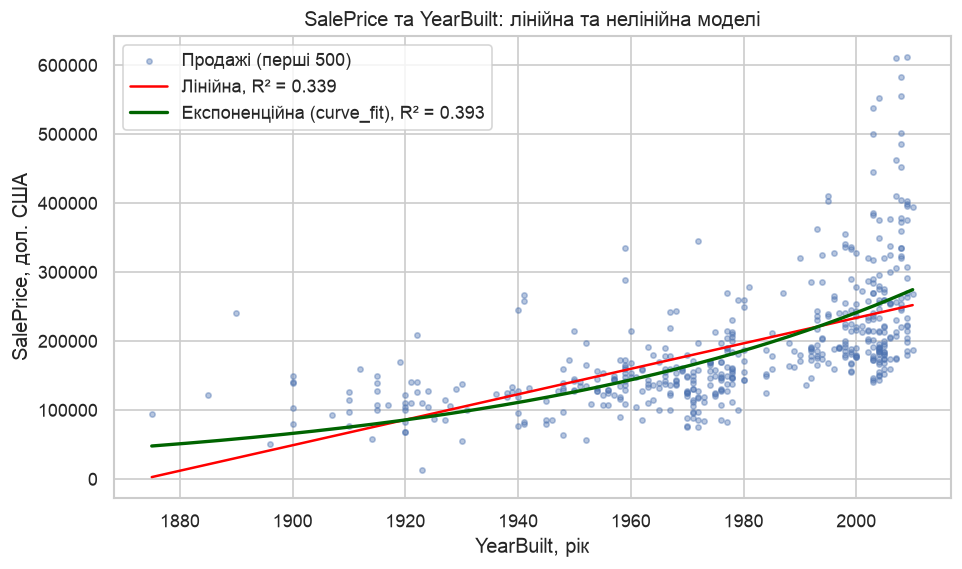
\includegraphics[width=\linewidth,height=0.82\textheight,keepaspectratio]{../../figures/problem6_nonlinear.png}
\caption{Порівняння лінійної та експоненційної моделей.}
\end{figure}


\answerheading
Модель: \[SalePrice_i=a\,e^{\,b\,(YearBuilt_i-1970)}+\varepsilon_i.\] де
\(a\) позначає ціну будинку 1970 року за моделлю, \(b\) темп зростання
за рік, \(\varepsilon_i\) похибку. Чому експонента: вона описує
зростання ціни на сталий відсоток за кожен пізніший рік будівництва, має
опуклу форму, як хмара точок, і за \(a>0\) дає додатні прогнозовані
ціни. Рік зсунуто на 1970 (близько до середнього 1977): тоді \(a\) є
прогнозом ціни будинку 1970 р., а обчислення стабільніші.

\texttt{curve\_fit} мінімізує
\[RSS(a,b)=\sum_i\big(y_i-a\,e^{\,b(x_i-1970)}\big)^2\] ітераційно (за
замовчуванням методом Левенберга--Марквардта), починаючи з початкових
значень \texttt{p0}; тут \(x_i\) позначає рік будівництва, а \(y_i\)
ціну продажу \(i\). Явної формули, як у лінійній регресії, немає.
\texttt{p0} взято з лінійної регресії \(\log(SalePrice)\) на
\((YearBuilt-1970)\): \(a_0=161996\), \(b_0=0.0102\).

Оцінки: \(\widehat a=163627\) дол. (прогноз для будинку 1970 р.),
\(\widehat b=0.01293\). Кожен пізніший рік будівництва збільшує прогноз
на \(100(e^{\widehat b}-1)=1.30\%\). Оцінка \(\widehat b\) більша за
початкову \(0.0102\). NLS мінімізує квадрати помилок у доларах, тож
дорогі нові будинки з великими відхиленнями важать більше; регресія
логарифма мінімізує квадрати логарифмічних помилок, які для малих
відхилень наближено відповідають відносним помилкам.

Порівняння на тих самих 500 продажах (обидві моделі мають по 2
параметри, тож скоригований \(R^2\) не потрібен):

\[R^2=1-\frac{\sum_i(y_i-\widehat y_i)^2}{\sum_i(y_i-\bar y)^2},\qquad MSE=\frac1n\sum_i(y_i-\widehat y_i)^2.\]
де \(\widehat y_i\) позначає прогноз відповідної моделі, \(\bar y\)
середню ціну, \(n=500\).

Експоненційна модель краща: MSE менша на 8.1\%, \(R^2\) вищий на 0.053.
Крива краще передає повільне зростання цін старих будинків і швидке
зростання цін нових. Для будинку 1880 р. вона прогнозує 51 тис. дол.
замість 12 тис. у прямої, для 2010 р. 275 тис. замість 252 тис.

Проте покращення помірне: обидві моделі пояснюють менше 40\% варіації,
бо ціну визначають також площа, якість, район тощо. Для нелінійної
моделі \(R^2\) є лише описовою мірою: розклад \(TSS=ESS+RSS\) тут не
виконується, і \(R^2\) навіть може бути від'ємним. Порівнювати \(R^2\)
двох моделей тут коректно, бо вони мають ті самі \(y\) і \(n\); це
рівнозначно порівнянню MSE.


\Needspace{186.0pt}

\subsection{(в) Статистичні висновки для NLS}

\begin{taskstatement}
Поясніть своїми словами, чому всі класичні тести та статистичні висновки
(наприклад, точні t-розподіли для малих вибірок) не є прямо застосовними
до оцінок нелінійного методу найменших квадратів (NLS), отриманих через
curve\_fit.
\end{taskstatement}


\pythoncode{p6-c12}

\begingroup\fontsize{7.5}{9.5}\selectfont\setlength{\tabcolsep}{2.5mm}\renewcommand{\arraystretch}{1.15}
\par\vspace{2pt}\noindent\begin{tabular}{|llllll|}
\hline
 & Оцінка & SE з pcov (наближена) & Оцінка / SE & Наближений 95\% ДІ: від & до \\
\hline
a & 163627 & 3854.67 & 42.449 & 156072 & 171182 \\
b & 0.0129343 & 0.000813133 & 15.9068 & 0.0113406 & 0.0145281 \\
\hline
\end{tabular}\par\vspace{2pt}
\endgroup


\Needspace{28.4pt}

\resulttext{p6-c12-out1.txt}

\begingroup\fontsize{7.5}{9.5}\selectfont\setlength{\tabcolsep}{2.5mm}\renewcommand{\arraystretch}{1.15}
\par\vspace{2pt}\noindent\begin{tabular}{|ll|}
\hline
 & Стандартне відхилення залишків, дол. \\
\hline
(1870, 1950] & 46474.6 \\
(1950, 1980] & 43587 \\
(1980, 2000] & 60448 \\
(2000, 2010] & 102347 \\
\hline
\end{tabular}\par\vspace{2pt}
\endgroup


\begin{figure}[H]
\centering
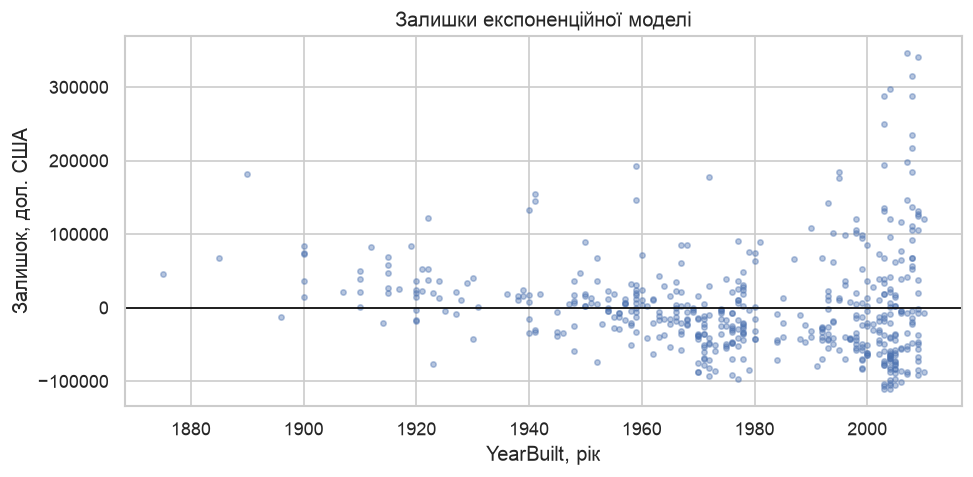
\includegraphics[width=\linewidth,height=0.82\textheight,keepaspectratio]{../../figures/problem6_residuals.png}
\caption{Залишки експоненційної моделі за роком будівництва.}
\end{figure}


\answerheading
Чому в лінійній регресії висновки точні. За фіксованих \(X\) оцінка
\[\widehat\beta=(X^TX)^{-1}X^Ty\] є лінійною функцією \(y\), де \(X\)
позначає матрицю регресорів, а \(y\) вектор відгуку. Якщо похибки
нормальні, \(\varepsilon\sim N(0,\sigma^2I)\), то \(\widehat\beta\)
точно нормальна, а \((n-k)s^2/\sigma^2\sim\chi^2(n-k)\) і не залежить
від \(\widehat\beta\). Тому
\(t=(\widehat\beta_j-\beta_j)/SE(\widehat\beta_j)\) має точний
t-розподіл для будь-якого \(n\), навіть \(n=10\). Так само точні й
F-тести.

Чому для NLS це не так. Оцінка
\(\widehat\theta=(\widehat a,\widehat b)\) не має формули: її знаходить
ітераційний алгоритм, і вона є нелінійною функцією \(y\). Навіть із
нормальними похибками \(\widehat\theta\) не є точно нормальною, у малих
вибірках може бути зміщеною, а \(s^2\) не має точного розподілу
\(\chi^2\). Тому точних t- і F-розподілів немає.

Що дає \texttt{curve\_fit}. Матриця \texttt{pcov} обчислюється через
лінеаризацію: біля \(\widehat\theta\) модель замінюють лінійною з
«регресорами»-похідними
\(J=\big[\partial f/\partial a,\ \partial f/\partial b\big]=\big[e^{bt},\ a\,t\,e^{bt}\big]\):
\[\widehat{Cov}(\widehat\theta)\approx s^2(J^TJ)^{-1},\qquad s^2=\frac{RSS}{n-2}.\]
де \(J\) позначає матрицю похідних, \(t=YearBuilt-1970\), \(s^2\) оцінку
дисперсії похибок, \(RSS\) суму квадратів залишків NLS. Це асимптотичне
наближення: воно добре, коли \(n\) велике, а модель майже лінійна в
межах невизначеності параметрів. Звідси \(SE(\widehat a)=3855\),
\(SE(\widehat b)=0.00081\) і наближений 95\% інтервал для \(b\):
\([0.0113;\ 0.0145]\), що після перетворення \(100(e^b-1)\) дає
приблизно 1.14--1.46\% за кожен пізніший рік будівництва. Тут ми свідомо
беремо нормальний квантиль 1.96, а не точний t-квантиль. Самих p-значень
\texttt{curve\_fit} не дає.

Наші дані додатково порушують припущення:

\begin{itemize}
\item
  залишки ненормальні: Jarque--Bera \(=672\), \(p\approx10^{-146}\);
\item
  розкид залишків зростає з роком: стандартне відхилення близько 44--46
  тис. дол. до 1980 р., 60 тис. у 1981--2000 рр. і 102 тис. після 2000
  р. (графік). Формула \texttt{pcov} припускає однакову дисперсію;
\item
  перші 500 рядків не є випадковою вибіркою.
\end{itemize}

Тому навіть наближені стандартні похибки й інтервали слід сприймати
обережно.


\Needspace{186.0pt}

\subsection{(г) Збіжність і перенавчання}

\begin{taskstatement}
Які проблеми з обчислювальною збіжністю (convergence) та перенавчанням
можуть виникнути, якщо ми вирішимо побудувати складну нелінійну
регресію, використовуючи одночасно всі наявні пояснювальні змінні у
датасеті?
\end{taskstatement}


\pythoncode{p6-c15}

\Needspace{37.599999999999994pt}

\resulttext{p6-c15-out0.txt}

\begingroup\fontsize{7.5}{9.5}\selectfont\setlength{\tabcolsep}{2.5mm}\renewcommand{\arraystretch}{1.15}
\par\vspace{2pt}\noindent\begin{tabular}{|llllll|}
\hline
 & a & SE(a) / a & b & Кореляція a і b & MSE \\
\hline
a*exp(b*(year - 1970)) & 163627 & 0.0235577 & 0.0129343 & -0.74794 & 4.84965e+09 \\
a*exp(b*year), добре p0 & 1.40509e-06 & 1.6199 & 0.0129344 & -0.999953 & 4.84965e+09 \\
\hline
\end{tabular}\par\vspace{2pt}
\endgroup


\begingroup\fontsize{7.5}{9.5}\selectfont\setlength{\tabcolsep}{2.5mm}\renewcommand{\arraystretch}{1.15}
\par\vspace{2pt}\noindent\begin{tabular}{|ll|}
\hline
 & Значення \\
\hline
Рядків & 500 \\
Стовпців після кодування категорій & 234 \\
Повних рядків (без NaN) & 393 \\
Стовпців, що в повних рядках завжди 0 & 16 \\
Стовпців, ненульових лише в 1 рядку & 19 \\
Ранг [1, X] на повних рядках & 204 \\
\hline
\end{tabular}\par\vspace{2pt}
\endgroup


\answerheading
Проблеми зі збіжністю.

\begin{itemize}
\item
  NLS не має явного розв'язку: алгоритм рухається від \texttt{p0} до
  мінімуму \(RSS(\theta)\). Ця функція може мати кілька локальних
  мінімумів і пласкі «долини». Алгоритм може зупинитися не там,
  розійтися або сильно залежати від \texttt{p0}. З усіма змінними
  параметрів сотні, і кожен крок потребує матриці похідних \(J\) розміру
  \(n\times p\). Підібрати добрі початкові значення для багатьох
  параметрів складніше; варто перевіряти кілька початкових наближень.
\item
  Навіть одна змінна показує проблему. Ту саму експоненту без зсуву
  року, \(a\,e^{b\cdot YearBuilt}\), запустили зі стандартним
  \texttt{p0\ =\ {[}1,\ 1{]}}. Тоді \(e^{1\cdot2000}\) переповнюється, і
  \texttt{curve\_fit} повернув \([1,1]\) без змін, з MSE \(=\infty\),
  лише з попередженнями, без помилки. З добрим \texttt{p0} ця версія
  знаходить ту саму криву (MSE однакова, \(4.85\cdot10^9\)). Але
  \(\widehat a=1.4\cdot10^{-6}\), відносна похибка \(\widehat a\) сягає
  162\%, а кореляція \(\widehat a\) і \(\widehat b\) дорівнює
  \(-0.99995\): такий запис чисельно незручний, а прогноз для року 0 є
  далекою екстраполяцією. Зі зсувом на 1970 кореляція \(-0.75\), а
  відносна похибка 2.4\%. Змінні Ames мають дуже різні масштаби (площі
  \textasciitilde{}\(10^4\), роки \textasciitilde2000, індикатори 0/1),
  тож таких проблем стане значно більше. Потрібні центрування й
  масштабування, обмеження на параметри, розумні \texttt{p0}.
\item
  Не всі параметри можна оцінити. Для перших 500 рядків кодування всіх
  змінних дає 234 стовпці. \texttt{curve\_fit} не приймає \texttt{NaN},
  а повних рядків лише 393. У цих рядках 16 індикаторів завжди
  дорівнюють 0, а 19 ненульові лише в одному рядку. Ранг матриці
  \([1, X]\) дорівнює 204 замість 235, тобто навіть лінійна модель не
  має єдиного розв'язку. Для конкретної нелінійної моделі треба окремо
  перевіряти ранг її якобіана \(J\): з рангу \(X\) він автоматично не
  випливає. Якщо стовпці \(J\) залежні, деякі параметри неможливо
  оцінити окремо; \texttt{curve\_fit} може видати попередження про
  коваріацію або дуже великі стандартні похибки.
\end{itemize}

Перенавчання.

\begin{itemize}
\item
  Потенційних параметрів багато відносно кількості спостережень (235
  стовпців на 393 повні рядки), а складні нелінійні форми можуть додати
  гнучкості. Зростає ризик підгонки шуму: навчальний \(R^2\) може бути
  високим, а помилка на нових будинках великою. Це ризик, а не
  гарантований результат; його перевіряють на відкладених даних або
  крос-валідацією.
\item
  У задачі 5 рідкісні категорії дали точну підгонку окремих будинків
  (\(h=1\)), а помилка крос-валідації була більшою за навчальну. Тут
  спостережень значно менше, тож діагностика рідкісних рівнів і
  перевірка прогнозів особливо важливі.
\end{itemize}

Що робити: обирати небагато змінних (відбір, як у задачі 5) і прості
форми, підказані графіками; часто достатньо лінійної моделі для
\(\log(SalePrice)\). Також допомагає регуляризація, а якість варто
перевіряти крос-валідацією, а не навчальним \(R^2\).

